% !TeX encoding = UTF-8
% !TeX program = xelatex
% !TeX spellcheck = en_US

\documentclass[a4paper]{article}
\usepackage{amsmath}
\usepackage[english]{babel}
\usepackage[UTF8]{ctex}
\usepackage{unicode-math}
\usepackage{caption}
\usepackage{booktabs}
\usepackage{xcolor}
\usepackage{array}
\usepackage{listings}
\usepackage{hypdoc}
\usepackage[left=0.50in,right=0.50in,top=1.0in,bottom=1.0in,paperheight=11in,paperwidth=8.5in]{geometry}
\usepackage{endnotes}
\usepackage{graphicx}
\usepackage{multicol}
\usepackage{float}
\usepackage{blindtext}
\usepackage{listings}
\usepackage{xcolor}
\lstset{frame=tb,
  language=Java,
  aboveskip=3mm,
  belowskip=3mm,
  showstringspaces=false,
  columns=flexible,
  basicstyle={\small\ttfamily},
  numbers=none,
  numberstyle=\tiny\color{gray},
  keywordstyle=\color{blue},
  commentstyle=\color{green},
  stringstyle=\color{purple},
  breaklines=true,
  breakatwhitespace=true,
  tabsize=3
}
\setlength{\columnsep}{1cm}
\title{Lab report:\\ Medical Physics view on temperature sensors}
\author{TiankaiMa PB21000030}
\date{\today}
\begin{document}
\begin{multicols*}{2}
  \maketitle
  \begin{abstract}
    Temperature is arguably the most important physical quantity in the area of medical physics. This lab report will give a brief introduction to how temperature sensors work and a measure of them.
    \par
    \textbf{Keywords:} Medical Physics, Temperature, Sensors, Thermometer
  \end{abstract}
  \section*{Introduction}
  Temperature sensors usually convert thermal information to electrical information, this is usually done with a thermistor, which has a changing resistance with temperature. This usually divides into three types: NTC(Negative Temperature Coefficient), PTC(Positive Temperature Coefficient), and CTC(Critical Temperature Coefficient). P-N junction diodes and LM35 sensors are also commonly used in temperature sensors.

  LM35, as its wide range of applications and extraordinary performance, is used in this experiment. In this lab report, we'll show how the LM35 sensor works in the lab environment, and calculate some of the parameters of the sensor.

  \section*{Methods}

  LM35 is packed in a T0-95 package, outputting voltage data corresponding to the temperature with great linearity, with a power source and voltmeter, we can calculate the temperature using the following equation:

  $$
    U_0 = Kt,\qquad U_0 \approx 10.0 mV/^\circ C
  $$

  Based on that equation and linear relationship, we can easily calculate \textbf{the level of sensitivity, correlation coefficient, and level of linearity}.

  \section*{Materials}
  \subsection*{Measure output characteristics}
  Connect the circuit add a Pt100 resistor and LM35 senor to the heating furnace, and turn on the switch.
  \par
  Starting from $30.0^\circ C$, the temperature is increased by $10.0^\circ C$ each time(up to $80.0^\circ C$), and the output voltage of the sensor is recorded. The level of sensitivity and correlation coefficient can be calculated using these data.

  \subsection*{Making a digital thermometer}
  Continue with the instruments used above, and connect the voltage sensor to an amplifying circuit. Compare the temperature shown on the voltmeter with the one from a thermometer and calibrate based on this. The steps are shown as the following:
  \par
  Calibrate both the Pt100 sensor and LM35 sensor with a digital thermometer at $30.0^\circ C$.(this is done with offset settings for the Pt100 and a potentiometer for the amplifying circuit that supports the LM35 sensor)
  \par
  To measure the level of linearity, raise the temperature from $35.0^\circ C$ to $42.0^\circ C$(with a step of $0.5^\circ C$), and record the temperature shown on the voltmeter. The level of linearity can be calculated using these data.

  \section*{Results}
  Results are attached in a separate paper.
  \newpage
  \section*{Discussion}
  \subsection*{Measure output characteristics}
  The linear relationship could be illustrated as the following:
  \begin{figure}[H]
    \centering
    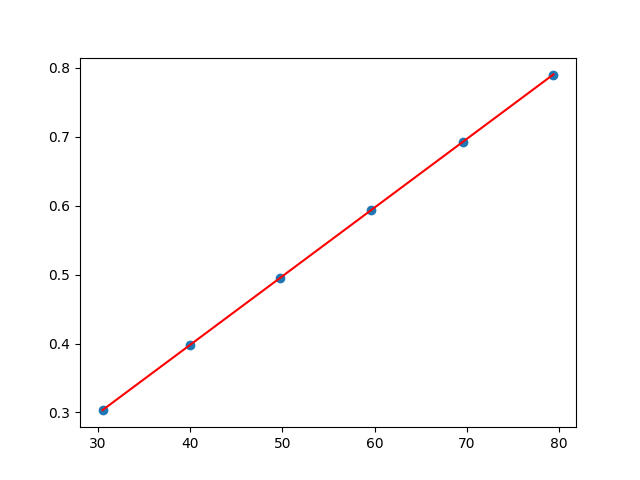
\includegraphics[width=0.8\linewidth]{./img/1.png}
    \caption{Voltage characteristics of LM35}
    \label{fig:figure1}
  \end{figure}
  \begin{equation*}
    \left\{
    \begin{aligned}
      r & = 0.99999                                       \\
      S & = 0.00995\ V/^\circ C \approx 10.0\ mV/^\circ C \\
    \end{aligned}
    \right.
  \end{equation*}
  \subsection*{Making a digital thermometer}
  The linear relationship could be illustrated as the following:
  \begin{figure}[H]
    \centering
    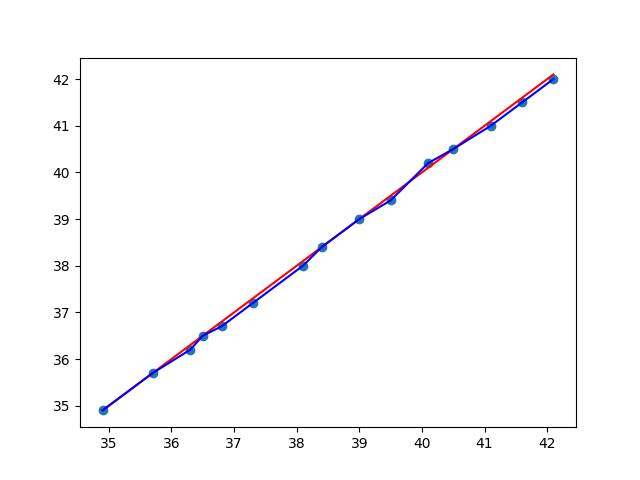
\includegraphics[width=0.8\linewidth]{./img/2.png}
    \caption{Difference between the temperature shown on the voltmeter and the thermometer}
    \label{fig:figure2}
  \end{figure}
  \begin{equation*}
    \delta = \Delta Y_{max} / Y = 0.0142
  \end{equation*}
  \section*{Conclusion}
  \begin{equation*}
    \left\{
    \begin{aligned}
      r      & = 0.99999                                       \\
      S      & = 0.00995\ V/^\circ C \approx 10.0\ mV/^\circ C \\
      \delta & = \Delta Y_{max} / Y = 0.0142                   \\
    \end{aligned}
    \right.
  \end{equation*}
  This experiment is a clear demonstration of LM35 and its excellent performance.
  \section*{References}
  \textit{Most contents were translated from the handout.}
  \section*{Code}
  The following code was used to make the graphics used:
  \begin{figure}[H]
    \centering
    \begin{lstlisting}[language=Python]
fit = np.polyfit(x, y, 1)
print(fit)
print(np.corrcoef(x,y))
plt.plot(x, fit[0] * x + fit[1])
plt.plot(x,x)
plt.plot(x,y)
plt.scatter(x, y)
plt.savefig('img/1.png')
\end{lstlisting}
  \end{figure}
\end{multicols*}
\end{document}